% Options for packages loaded elsewhere
\PassOptionsToPackage{unicode}{hyperref}
\PassOptionsToPackage{hyphens}{url}
\PassOptionsToPackage{dvipsnames,svgnames,x11names}{xcolor}
%
\documentclass[
  11pt,
]{article}

\usepackage{amsmath,amssymb}
\usepackage{iftex}
\ifPDFTeX
  \usepackage[T1]{fontenc}
  \usepackage[utf8]{inputenc}
  \usepackage{textcomp} % provide euro and other symbols
\else % if luatex or xetex
  \usepackage{unicode-math}
  \defaultfontfeatures{Scale=MatchLowercase}
  \defaultfontfeatures[\rmfamily]{Ligatures=TeX,Scale=1}
\fi
\usepackage{lmodern}
\ifPDFTeX\else  
    % xetex/luatex font selection
    \setmainfont[]{Century Gothic}
\fi
% Use upquote if available, for straight quotes in verbatim environments
\IfFileExists{upquote.sty}{\usepackage{upquote}}{}
\IfFileExists{microtype.sty}{% use microtype if available
  \usepackage[]{microtype}
  \UseMicrotypeSet[protrusion]{basicmath} % disable protrusion for tt fonts
}{}
\makeatletter
\@ifundefined{KOMAClassName}{% if non-KOMA class
  \IfFileExists{parskip.sty}{%
    \usepackage{parskip}
  }{% else
    \setlength{\parindent}{0pt}
    \setlength{\parskip}{6pt plus 2pt minus 1pt}}
}{% if KOMA class
  \KOMAoptions{parskip=half}}
\makeatother
\usepackage{xcolor}
\setlength{\emergencystretch}{3em} % prevent overfull lines
\setcounter{secnumdepth}{-\maxdimen} % remove section numbering
% Make \paragraph and \subparagraph free-standing
\makeatletter
\ifx\paragraph\undefined\else
  \let\oldparagraph\paragraph
  \renewcommand{\paragraph}{
    \@ifstar
      \xxxParagraphStar
      \xxxParagraphNoStar
  }
  \newcommand{\xxxParagraphStar}[1]{\oldparagraph*{#1}\mbox{}}
  \newcommand{\xxxParagraphNoStar}[1]{\oldparagraph{#1}\mbox{}}
\fi
\ifx\subparagraph\undefined\else
  \let\oldsubparagraph\subparagraph
  \renewcommand{\subparagraph}{
    \@ifstar
      \xxxSubParagraphStar
      \xxxSubParagraphNoStar
  }
  \newcommand{\xxxSubParagraphStar}[1]{\oldsubparagraph*{#1}\mbox{}}
  \newcommand{\xxxSubParagraphNoStar}[1]{\oldsubparagraph{#1}\mbox{}}
\fi
\makeatother


\providecommand{\tightlist}{%
  \setlength{\itemsep}{0pt}\setlength{\parskip}{0pt}}\usepackage{longtable,booktabs,array}
\usepackage{calc} % for calculating minipage widths
% Correct order of tables after \paragraph or \subparagraph
\usepackage{etoolbox}
\makeatletter
\patchcmd\longtable{\par}{\if@noskipsec\mbox{}\fi\par}{}{}
\makeatother
% Allow footnotes in longtable head/foot
\IfFileExists{footnotehyper.sty}{\usepackage{footnotehyper}}{\usepackage{footnote}}
\makesavenoteenv{longtable}
\usepackage{graphicx}
\makeatletter
\def\maxwidth{\ifdim\Gin@nat@width>\linewidth\linewidth\else\Gin@nat@width\fi}
\def\maxheight{\ifdim\Gin@nat@height>\textheight\textheight\else\Gin@nat@height\fi}
\makeatother
% Scale images if necessary, so that they will not overflow the page
% margins by default, and it is still possible to overwrite the defaults
% using explicit options in \includegraphics[width, height, ...]{}
\setkeys{Gin}{width=\maxwidth,height=\maxheight,keepaspectratio}
% Set default figure placement to htbp
\makeatletter
\def\fps@figure{htbp}
\makeatother

\usepackage{booktabs}
\usepackage{longtable}
\usepackage{array}
\usepackage{multirow}
\usepackage{wrapfig}
\usepackage{float}
\usepackage{colortbl}
\usepackage{pdflscape}
\usepackage{tabu}
\usepackage{threeparttable}
\usepackage{threeparttablex}
\usepackage[normalem]{ulem}
\usepackage{makecell}
\usepackage{xcolor}
\usepackage{fancyhdr}
\pagestyle{fancy}
\fancyhf{}
\rfoot{\thepage}
\floatplacement{figure}{H}
\floatplacement{table}{H}
\usepackage{geometry}
\geometry{ left=1.5cm, right=1.5cm, top=2.5cm, bottom=2.5cm }
\usepackage{flafter}
\raggedbottom
\usepackage{placeins}
\usepackage{ragged2e}
\usepackage{float}
\usepackage{setspace}
\renewcommand{\familydefault}{\sfdefault}
\AtBeginDocument{\renewcommand{\baselinestretch}{1.5}\justifying}
\fancyhead[LO,RE]{}
\fancyhead[LE,RO]{}
\makeatletter
\@ifpackageloaded{caption}{}{\usepackage{caption}}
\AtBeginDocument{%
\ifdefined\contentsname
  \renewcommand*\contentsname{Tabla de contenidos}
\else
  \newcommand\contentsname{Tabla de contenidos}
\fi
\ifdefined\listfigurename
  \renewcommand*\listfigurename{Listado de Figuras}
\else
  \newcommand\listfigurename{Listado de Figuras}
\fi
\ifdefined\listtablename
  \renewcommand*\listtablename{Listado de Tablas}
\else
  \newcommand\listtablename{Listado de Tablas}
\fi
\ifdefined\figurename
  \renewcommand*\figurename{Figura}
\else
  \newcommand\figurename{Figura}
\fi
\ifdefined\tablename
  \renewcommand*\tablename{Tabla}
\else
  \newcommand\tablename{Tabla}
\fi
}
\@ifpackageloaded{float}{}{\usepackage{float}}
\floatstyle{ruled}
\@ifundefined{c@chapter}{\newfloat{codelisting}{h}{lop}}{\newfloat{codelisting}{h}{lop}[chapter]}
\floatname{codelisting}{Listado}
\newcommand*\listoflistings{\listof{codelisting}{Listado de Listados}}
\makeatother
\makeatletter
\makeatother
\makeatletter
\@ifpackageloaded{caption}{}{\usepackage{caption}}
\@ifpackageloaded{subcaption}{}{\usepackage{subcaption}}
\makeatother

\ifLuaTeX
\usepackage[bidi=basic]{babel}
\else
\usepackage[bidi=default]{babel}
\fi
\babelprovide[main,import]{spanish}
\ifPDFTeX
\else
\babelfont{rm}[]{Century Gothic}
\fi
% get rid of language-specific shorthands (see #6817):
\let\LanguageShortHands\languageshorthands
\def\languageshorthands#1{}
\ifLuaTeX
  \usepackage{selnolig}  % disable illegal ligatures
\fi
\usepackage{bookmark}

\IfFileExists{xurl.sty}{\usepackage{xurl}}{} % add URL line breaks if available
\urlstyle{same} % disable monospaced font for URLs
\hypersetup{
  pdftitle={Reporte},
  pdfauthor={Cliodinámica},
  pdflang={es},
  colorlinks=true,
  linkcolor={blue},
  filecolor={Maroon},
  citecolor={Blue},
  urlcolor={Blue},
  pdfcreator={LaTeX via pandoc}}


\title{Reporte}
\author{Cliodinámica}
\date{}

\begin{document}
\maketitle


\newpage

\centering


\includegraphics[width=0.5\textwidth]{Imagenes/color_MinTrabajo.png}
\vspace{2cm}

\noindent Ministerio del Trabajo y Previsión Social

División de Políticas de Empleo\textbackslash{} Subsecretaría del
Trabajo

\justifying

El presente documento analiza los resultados de la Encuesta Nacional de
Demanda Laboral (ENADEL) 2023, que busca identificar y caracterizar el
capital humano requerido por las empresas de los distintos sectores
productivos del país, generando información sobre la demanda actual de
ocupaciones de las empresas, detectando requisitos y problemas de
contratación. Al igual que versiones anteriores de esta encuesta, se
puso el foco en dos sectores de actividad económica: Construcción y el
sector Agrícola.

\newpage
\renewcommand{\contentsname}{Índice} 
\tableofcontents

\newpage

\subsection{Descripción General: Empresas y
Trabajadores}\label{descripciuxf3n-general-empresas-y-trabajadores}

La muestra de ENADEL 2023 encuesta a 5.820 empresas que suman 485.256
trabajadores (a nivel muestral). Estas representan a 82.052 empresas y
5.611.196 trabajadores a nivel nacional. La Tabla~\ref{tbl-region}
muestra la distribución en las distintas regiones del país, dónde un
\text{53,6}\% de las empresas y un \text{65,6}\% de los trabajadores se
encuentran en la región Metropolitana.

\vspace{-5mm}

\FloatBarrier

\begin{table}

\caption{\label{tbl-region}Resultados de la encuesta}

\centering{

[!h]
\centering\centering
\begin{tabular}{lrr}
\toprule
Región & \% Empresas & \% Trabajadores\\
\midrule
Arica y Parinacota & 0,67 & 0,33\\
Tarapacá & 1,69 & 1,07\\
Antofagasta & 2,60 & 1,82\\
Atacama & 0,76 & 0,54\\
Coquimbo & 2,78 & 1,86\\
\addlinespace
Valparaíso & 9,05 & 6,50\\
Metropolitana & 53,61 & 65,59\\
O'Higgins & 5,10 & 4,21\\
Maule & 1,54 & 1,01\\
Ñuble & 6,66 & 4,96\\
\addlinespace
Biobío & 1,35 & 0,69\\
Araucanía & 4,59 & 3,45\\
Los Ríos & 0,39 & 0,25\\
Los Lagos & 0,98 & 0,64\\
Aysén & 4,92 & 4,74\\
\addlinespace
Magallanes & 3,30 & 2,34\\
\bottomrule
\multicolumn{3}{l}{\rule{0pt}{1em}Fuente: Elaboración propia utilizando datos de ENADEL 2023.}\\
\end{tabular}

}

\end{table}%

\FloatBarrier

La Figura~\ref{fig-combined} muestra el porcentaje de empresas y
trabajadores según tamaño de empresas, utilizando la clasificación por
número de trabajadores, cómo por volumen de venta. Con respecto a la
primera clasificación, el 74,6\% de las empresas tiene menos de 50
trabajadores --acumulando un 23,8\% del total-- y casi el 50\% de los
trabajadores están en empresas grandes --que corresponden a un 6,5\% del
total. Si se analiza según tamaño de ventas, más de la mitad de las
empresas tienen un volumen de venta de entre 2.400 y 24.999 UF
(``Pequeñas'') y más de un cuarto venden entre 25.000 y 100.000 UF al
año (``Mediana''). Sin embargo, casi un tercio de los trabajadores están
en empresas grandes (más de 100.000 UF).

\FloatBarrier

\begin{figure}[H]

\caption{\label{fig-combined}Gráfico combinado de resultados}

\centering{

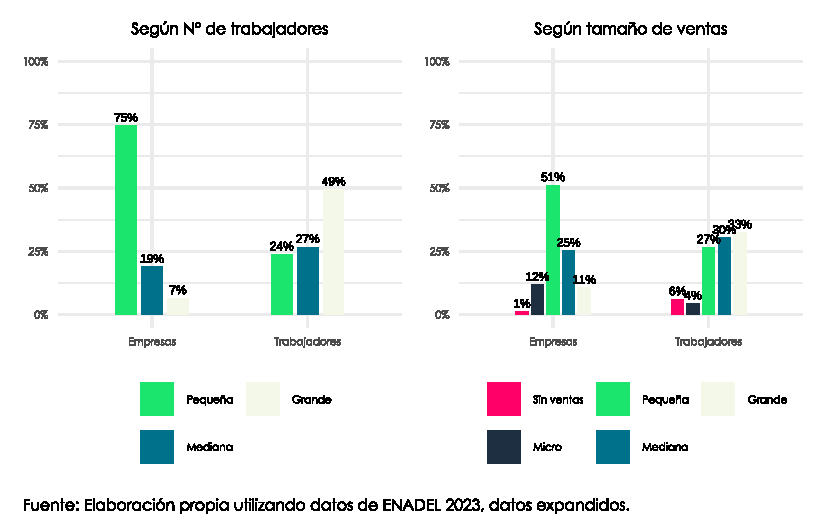
\includegraphics[width=1\textwidth,height=\textheight]{Reporte_files/figure-pdf/fig-combined-1.pdf}

}

\end{figure}%

\FloatBarrier

Al revisar la distribución por sector de actividad económica
Tabla~\ref{tbl-acteco} se tiene que una de cada cinco empresas pertenece
al sector de Comercio, seguido por el sector Construcción
(\text{15,5}\%) y el sector de Industrias Manufactureras (11,4\%). Con
respecto al volumen de trabajadores, el sector Comercio también lidera
(17,8\%) seguido por el sector Construcción (14,4\%) y el sector de
Servicios Administrativos y de Apoyo que, siendo sector intensivo en
trabajo, un 9,1\% de las empresas acumula el 13,5\% de trabajadores y
trabajadoras.

\FloatBarrier

\begin{table}

\caption{\label{tbl-acteco}Empresas y trabajadores según sector de
actividad económica}

\centering{

\centering
\begin{tabular}{lrr}
\toprule
Actividad Económica & \% Empresas & \% Trabajadores\\
\midrule
Comercio & 20,60 & 17,78\\
Construcción & 15,54 & 14,42\\
Servicios administrativos y de apoyo & 9,08 & 13,50\\
Industria manufacturera & 11,39 & 11,81\\
Actividades profesionales & 10,82 & 10,97\\
\addlinespace
Silvoagropecuario & 8,64 & 8,33\\
Transporte y almacenamiento & 7,62 & 5,91\\
Administración pública & 0,69 & 5,46\\
Alojamiento y de servicio de comidas & 6,79 & 4,03\\
Información y comunicaciones & 3,02 & 2,61\\
\addlinespace
Actividades inmobiliarias & 3,15 & 2,60\\
Actividades financieras y de seguros & 1,88 & 1,69\\
Pesca y acuicultura & 0,77 & 0,90\\
\bottomrule
\multicolumn{3}{l}{\rule{0pt}{1em}Fuente: Elaboración propia utilizando datos de ENADEL 2023.}\\
\end{tabular}

}

\end{table}%

\FloatBarrier

\subsubsection{Contratados en los últimos 12
meses}\label{contratados-en-los-uxfaltimos-12-meses}

El 87,1\% de las empresas declaró que sí contrató personas nuevas
durante los últimos 12 meses, mientras que el 12,9\% declara que no
contrató personas nuevas durante el mismo período. La
Tabla~\ref{tbl-contratos_totales} muestra la proporción de empresas,
según sector de actividad económica, que tuvieron contrataciones nuevas
durante los últimos 12 meses. El 98.9\% de las empresas del sector de
pesca y acuicultura respondieron afirmativamente, mientras que el sector
con menor proporción fue el de Actividades Inmobiliarias, dónde el
24,9\% de firmas no tuvieron contrataciones durante los últimos 12
meses.

\FloatBarrier

\begin{table}

\caption{\label{tbl-contratos_totales}}

\centering{

\centering
\begin{tabular}{lrr}
\toprule
Actividad Económica & \% Si & \% No\\
\midrule
Actividades profesionales & 90,4 & 9,6\\
Actividades financieras y de seguros & 83,9 & 16,1\\
Actividades inmobiliarias & 75,1 & 24,9\\
Administración pública & 90,3 & 9,7\\
Alojamiento y de servicio de comidas & 92,9 & 7,1\\
\addlinespace
Comercio & 84,8 & 15,2\\
Construcción & 89,3 & 10,7\\
Industria manufacturera & 87,3 & 12,7\\
Información y comunicaciones & 90,3 & 9,7\\
Servicios administrativos y de apoyo & 87,5 & 12,5\\
\addlinespace
Silvoagropecuario & 83,6 & 16,4\\
Pesca y acuicultura & 98,9 & 1,1\\
Transporte y almacenamiento & 85,0 & 15,0\\
\bottomrule
\multicolumn{3}{l}{\rule{0pt}{1em}Fuente: Elaboración propia utilizando datos de ENADEL 2023.}\\
\end{tabular}

}

\end{table}%

\FloatBarrier

\subparagraph{Contrataciones por
ocupación}\label{contrataciones-por-ocupaciuxf3n}

\subparagraph{Contrataciones por ocupación: Sector
Construcción}\label{contrataciones-por-ocupaciuxf3n-sector-construcciuxf3n}

\subparagraph{Contrataciones por ocupación: Sector
Agrícola}\label{contrataciones-por-ocupaciuxf3n-sector-agruxedcola}

\subsubsection{Vacantes en los últimos 12
meses}\label{vacantes-en-los-uxfaltimos-12-meses}

\subparagraph{Ocupaciones de difícil
cobertura}\label{ocupaciones-de-difuxedcil-cobertura}

\subparagraph{Ocupaciones de Difícil Cobertura: Sector
Construcción}\label{ocupaciones-de-difuxedcil-cobertura-sector-construcciuxf3n}

\subparagraph{Ocupaciones de Difícil Cobertura: Sector
Agrícola}\label{ocupaciones-de-difuxedcil-cobertura-sector-agruxedcola}

\subsubsection{Dificultades para la
contratación}\label{dificultades-para-la-contrataciuxf3n}

\subparagraph{Dificultades para la contratación: Sector
Construcción}\label{dificultades-para-la-contrataciuxf3n-sector-construcciuxf3n}

\subparagraph{Dificultades para la contratación: Sector
Agrícola}\label{dificultades-para-la-contrataciuxf3n-sector-agruxedcola}

\subsubsection{Educación y
experiencia}\label{educaciuxf3n-y-experiencia}

\subsubsection{Canales de reclutamiento}\label{canales-de-reclutamiento}

\subsubsection{Conocimiento de instituciones y
programas}\label{conocimiento-de-instituciones-y-programas}

\subsubsection{Apéndice A: Ocupaciones de Difícil
Cobertura}\label{apuxe9ndice-a-ocupaciones-de-difuxedcil-cobertura}




\end{document}
